%%%%%%%%%%%%%%%%%%%%%%%%%%%%%%%%%%%%%%%%%%%%%%%%%%%%%%%%%%%%%%%%%%%%%%%%
%     LaTeX source code to approximate a Draft NIST Technical report
%	  Instructions for authors: tinyurl.com/techpubsnist 
%	DOI watermark will be added on final PDF
% 	Developed by K. Miller, kmm5@nist.gov 
%	Last updated: 22-March-2019
%%%%%%%%%%%%%%%%%%%%%%%%%%%%%%%%%%%%%%%%%%%%%%%%%%%%%%%%%%%%%%%%%%%

%%%%%%%%%%%%%%%%%%%%%%
% Template further altered by Armen Amirkhanian
% for use with UA lab courses in an effort to 
% have a standardized format for lab documents
% Last update 9-April-2020
%
% TODO:
% --Get the appendices to dynamically link, tocloft causes problems
%%%%%%%%%%%%%%%%%%%%%%

\documentclass[12pt]{article}
\usepackage{amsmath}
\usepackage{amsfonts}   % if you want the fonts
\usepackage{amssymb}    % if you want extra symbols
\usepackage{graphicx}   % need for figures
\usepackage{xcolor}
\usepackage{bm}
\usepackage{secdot}		
\usepackage{mathptmx}
\usepackage{float}
\usepackage[utf8]{inputenc}
\usepackage{textcomp}
\usepackage[hang,flushmargin,bottom]{footmisc} % footnote format
\usepackage{xspace}
%\usepackage{lineno}
\usepackage{ragged2e}
\usepackage{parskip}
\usepackage{textcomp}

\usepackage{tikz}
\usetikzlibrary{shapes.geometric, arrows}
\tikzstyle{startstop} = [rectangle, rounded corners, minimum width=2cm, minimum height=1cm,text centered, draw=black, fill=red!20]
\tikzstyle{arrow} = [thick,->,>=stealth]

\usepackage{titlesec}
\titleformat{\section}{\normalsize\bfseries}{\thesection.}{1em}{}	% required for heading numbering style
\titleformat*{\subsection}{\normalsize\bfseries}

\usepackage{tocloft}	% change typeset, titles, and format list of appendices/figures/tables
\renewcommand{\cftdot}{}	
\renewcommand{\contentsname}{Table of Contents}
\renewcommand{\cftpartleader}{\cftdotfill{\cftdotsep}} % for parts
\renewcommand{\cftsecleader}{\cftdotfill{\cftdotsep}}
\renewcommand\cftbeforesecskip{\setlength{4pt}{}}
\addtolength{\cftfignumwidth}{1em}
\renewcommand{\cftfigpresnum}{\figurename\ }
\addtolength{\cfttabnumwidth}{1em}
\renewcommand{\cfttabpresnum}{\tablename\ }
\setlength{\cfttabindent}{0in}    %% adjust as you like
\setlength{\cftfigindent}{0in} 

\usepackage{enumitem}         % to control spacing between bullets/numbered lists

\usepackage[numbers,sort&compress]{natbib} % format bibliography 
\renewcommand{\bibsection}{}
\setlength{\bibsep}{0.0pt}

\usepackage[hidelinks]{hyperref}
\hypersetup{
	colorlinks = true,
urlcolor ={blue},
citecolor = {.},
linkcolor = {.},
anchorcolor = {.},
filecolor = {.},
menucolor = {.},
runcolor = {.}
pdftitle={},
pdfsubject={},
pdfauthor={},
pdfkeywords={}
}
\urlstyle{same}

\usepackage{epstopdf} % converting EPS figure files to PDF

\usepackage{fancyhdr, lastpage}	% formatting document, calculating number of pages, formatting headers
\setlength{\topmargin}{-0.5in}
\setlength{\headheight}{39pt}
\setlength{\oddsidemargin}{0.25in}
\setlength{\evensidemargin}{0.25in}
\setlength{\textwidth}{6.0in}
\setlength{\textheight}{8.5in}

\usepackage{caption} % required for Figure labels
\captionsetup{font=small,labelfont=bf,figurename=Fig.,labelsep=period,justification=raggedright} 

%%%%%%%%%%% !!!!!REQUIRED - FILL OUT METADATA HERE !!!!!!!! %%%%%%%%%%%%%%
%%%%%%%%%%%%%%%%%%%%%%%%%%%%%%%%%%%%%%%%%%%%%%%%%%%%%%%%%%%%%%%%%%%%%%%%%%
\newcommand{\CourseNum}{CE340}
\newcommand{\CourseName}{Geotechnical Engineering}
\newcommand{\LabTitle}{Atterberg Limits}
\newcommand{\LastUpdate}{Summer 2020}

%%%%%%%%%%%%%%%%%%%%%%%%%%%%%%%%%%%%%%%%%%%%%%%%%%%%%%%%%%%%%%%%%%%%
%   	BEGIN DOCUMENT 
%%%%%%%%%%%%%%%%%%%%%%%%%%%%%%%%%%%%%%%%%%%%%%%%%%%%%%%%%%%%%%%%%%%%
\begin{document}
	\urlstyle{rm} % Format style of \url   
%\linenumbers
\begin{titlepage}
\begin{flushright}
\LARGE{\textbf{\CourseNum{} -- \CourseName}}\\
\vfill
\Huge{\textbf{\LabTitle}}\\
    \vfill
%%%%%%%%%%%%%%%%%%%%%%%%%%%%%%%%%%%%%%%%%%%%%%%%%%%%%%%%%%%%%%%%%%%%
%	Authors - add complete list of authors, affiliations will be 
%   added on title page
%%%%%%%%%%%%%%%%%%%%%%%%%%%%%%%%%%%%%%%%%%%%%%%%%%%%%%%%%%%%%%%%%%%%
    \large Dr. Armen Amirkhanian, P.E.\\
    \normalsize Dr. Olugbenro Ogunrinde (Reviewer)\\
    \normalsize Sam Prather (Reviewer)\\
    \normalsize Eleanor ``Lea'' Skelton, P.E. (Reviewer)\\
\vfill
%%%%%%%%%%%%%%%%%%%%%%%%%%%%%%%%%%%%%%%%%%%%%%%%%%%%%%%%%%%%%%%%%%%%
%	The DOI is automated based on metadata.	
%%%%%%%%%%%%%%%%%%%%%%%%%%%%%%%%%%%%%%%%%%%%%%%%%%%%%%%%%%%%%%%%%%%%
\normalsize This work is licensed under the Creative Commons Attribution-ShareAlike 4.0 International License. To view a copy of this license, visit:
\href{http://creativecommons.org/licenses/by-sa/4.0/}{http://creativecommons.org/licenses/by-sa/4.0/}.


\includegraphics[width=0.07\textwidth]{cc.eps}
\includegraphics[width=0.07\textwidth]{by.eps}

\includegraphics[width=0.07\textwidth]{sa.eps}
\vfill

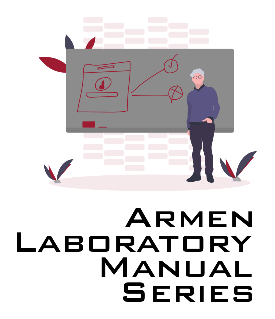
\includegraphics[width=0.3\linewidth]{Logo.eps}\\ 
 
  
\end{flushright}
\end{titlepage}

\begin{titlepage}
\begin{center}
\normalsize 
Certain commercial entities, equipment, or materials may be identified in this document in order to describe an experimental procedure or concept adequately. Such identification is not intended to imply recommendation or endorsement by The University of Alabama or the listed authors, nor is it intended to imply that the entities, materials, or equipment are necessarily the best available for the purpose.\\

\vfill
Any opinions or recommendations are solely those of the authors and do not represent the official view or policy of The University of Alabama.
\end{center}
\begin{flushright}
\vfill
\normalsize 
This document was last updated in \textbf{\LastUpdate} and should contain \textbf{\pageref{LastPage}} pages of content exclusive of these title pages, abstract, and other front matter. If the document appears to be incomplete, please contact the author(s).\\
\vfill
I am, and ever will be, a white-socks, pocket-protector, nerdy engineer...\\
\textit{Neil Armstrong}
\end{flushright}
\end{titlepage}
%%%%%%%%%%%%%%%%%%%%%%%%%%%%%%%%%%%%%%%%%%%%%%%%%%%%%%%%%%%%%%%%%%%%
%   Start front matter - page number starts with "i"
%%%%%%%%%%%%%%%%%%%%%%%%%%%%%%%%%%%%%%%%%%%%%%%%%%%%%%%%%%%%%%%%%%%%
\pagenumbering{roman}
\section*{Abstract}
\normalsize Atterberg limits describe a soil's response to changing moisture conditions. There were six limits originally defined by Albert Atterberg in the early 1900s. However, the two that are most important in civil engineering applications are the plastic limit and liquid limit. The plastic limit corresponds to the moisture state in which the soil transitions from a semi-solid state to a plastic state. The liquid limit corresponds to the moisture state in which the soil transitions from a plastic state to a liquid state. These two parameters can then be used to calculate a plasticity index which is used in soil classification. Additionally, the engineering behavior of soils has been well correlated to these limits and index and provides a quick gut check for the expected behavior for a soil.\\

\vfill
\section*{Keywords}
\normalsize atterberg limits; plastic limit; liquid limit; plasticity index; soil classification.\\
\pagebreak
%%%%%%%%%%%%%%%%%%%%%%%%%%%%%%%%%%%%%%%%%%%%%%%%%%%%%%%%%%%%%%%%%%%%
%   Table of Contents is required
% 	List of Tables & Figures required if more than 5 tables/figures
%%%%%%%%%%%%%%%%%%%%%%%%%%%%%%%%%%%%%%%%%%%%%%%%%%%%%%%%%%%%%%%%%%%%
\begin{center}
\tableofcontents
\pagebreak
\listoftables
\listoffigures
\end{center}
\pagebreak
\section*{Required Specifications}
The following specifications are required to complete this laboratory exercise:
\begin{description}
\item[ASTM D2487] Practice for Classification of Soils for Engineering Purposes (Unified Soil Classification System)
\item[ASTM D4318] Standard Test Methods for Liquid Limit, Plastic Limit, and Plasticity Index of Soils
\end{description}

The following specifications are optional, but they are listed here in the event more information is needed to complete the laboratory exercise:
\begin{description}
\item[ASTM D6026] Standard Practice for Using Significant Digits in Geotechnical Data
\item[ASTM E11] Specification for Woven Wire Test Sieve Cloth and Test Sieves
\end{description}
\pagebreak
%%%%%%%%%%%%%%%%%%%%%%%%%%%%%%%%%%%%%%%%%%%%%%%%%%%%%%%%%%%%%%%%%%%%
%   Start body of text - page number starts with "1"
%%%%%%%%%%%%%%%%%%%%%%%%%%%%%%%%%%%%%%%%%%%%%%%%%%%%%%%%%%%%%%%%%%%%
\section{Plastic Limit Test}
\label{sec:intro}
\pagenumbering{arabic}
\normalsize 
The plastic limit test is a relatively simple test that requires almost no equipment. A sample of moist soil is rolled into a string. When the string reaches the required diameter and is just beginning to break apart, the moisture content is measured. This test identifies the transition between a semi-solid state to a plastic state. Think of it like the transition between Play-Doh\textregistered{} that has been left out for a day (i.e. semi-solid) to brand new Play-Doh\textregistered{} (i.e. plastic). Students often misinterpret the term ``plastic'', thinking it means something hard and rigid. However, we are using the term ``plastic'' to indicate that if we deform the material, the deformation is permanent, that is ``plastic'', but it does not fracture or break the specimen to any noticeable degree. This test is typically performed on fine grained soils or the fine grained portion of mixed soils. Soils with insufficient cohesion to be rolled are considered non-plastic and are classified as silts.

\subsection{Objectives}
\label{ssec:headingscap}
At the completion of this lab exercise, you will have satisfied the following objectives:
\begin{enumerate}
    \item Perform a series of plastic limit tests on a silty-clayey soil material
    \item Perform calculations necessary to determine the plastic limit
\end{enumerate}

\subsection{Learning Outcomes}
At the completion of this lab exercise, you should be able to:
\begin{itemize}
    \item understand the difference between semi-solid and plastic state of a soil material
    \item perform calculations necessary to determine the plastic limit of a soil material
\end{itemize}

\pagebreak
\subsection{Procedure}
The plastic limit test procedure is divided into three parts: preparation, execution, and analysis. ASTM D4318 \S16.1 requires that the sample used for the plastic limit test be from the liquid limit test. However, for purposes of this lab, you will use a separately conditioned sample. You will repeatedly evaluate the material until it reaches a consistency at which it can be molded in your hands without sticking. The you will roll it into a string. This will be done at several moisture contents and the one at which it just begins to crumble is the plastic limit.

\subsubsection{Preparation}
You will need four pieces of equipment for this procedure: glass plate, a comparison rod that has a 3.2 mm diameter, two sample containers (Fig. \ref{fig:samplecontainer}), and a scale. This glass plate provides a smooth surface upon which to roll out your soil sample. The comparison rod will assist you in determining if your rolled sample is of the correct diameter.

\begin{figure}[H]
    \centering
    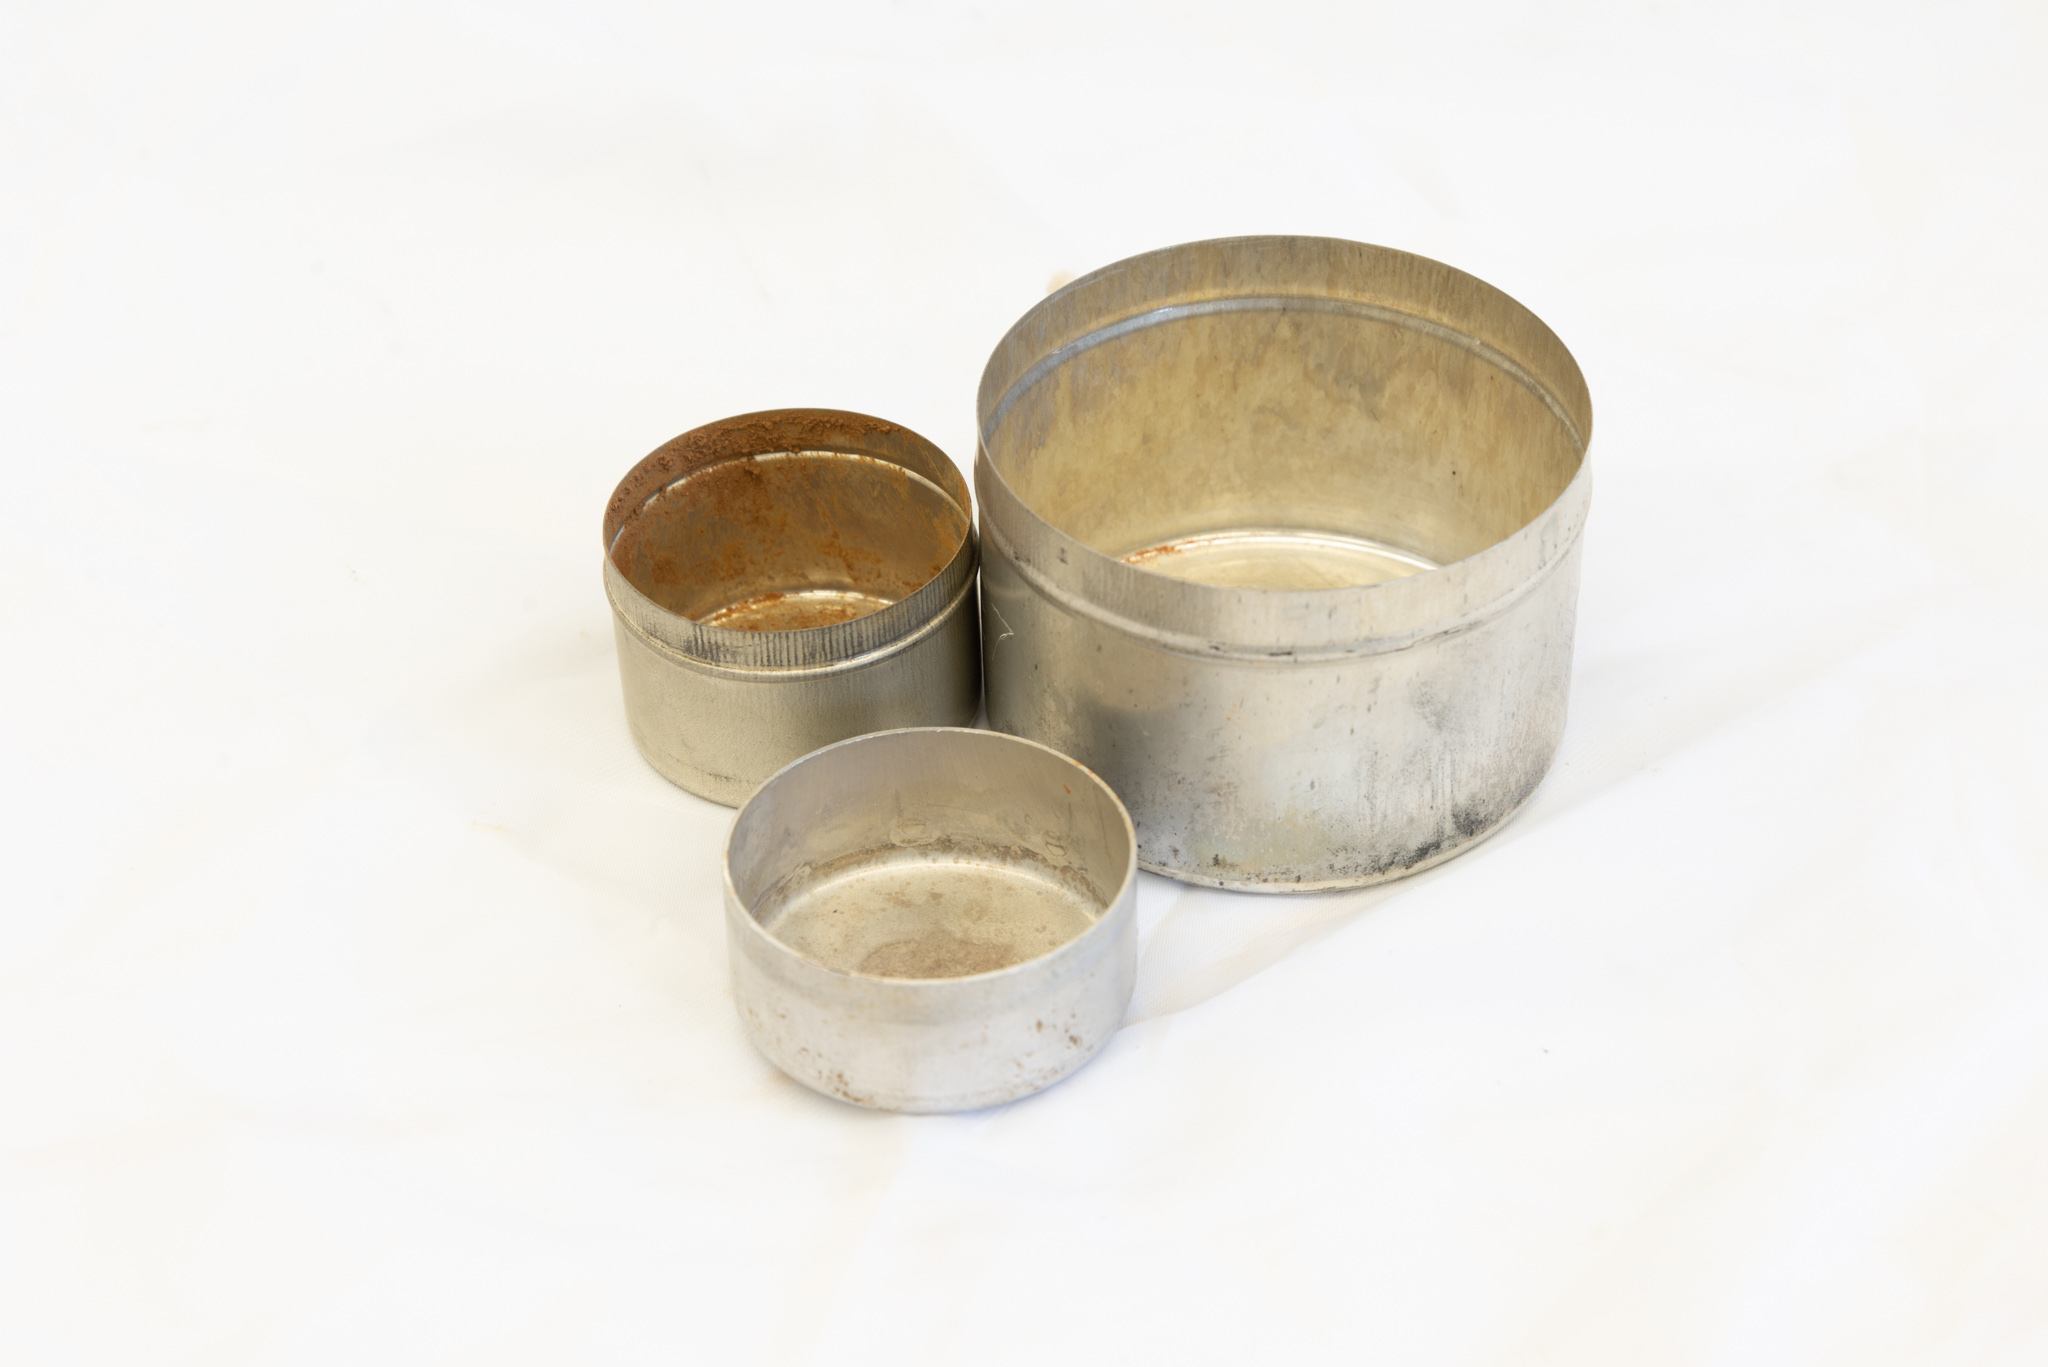
\includegraphics[width=0.8\textwidth]{GEO_5749.jpg}
    \caption{Aluminum sample containers that can be used for Atterberg limit tests. There is no requirement on the required size of the sample can, just that it can sufficiently hold the material to be oven dried.}
    \label{fig:samplecontainer}
\end{figure}

You will also need about 20 g of prepared soil. You should note that the provided soil material completely passes the \#40 sieve (425 $\mu$m). Your hands at this time should be clean and dry. Finally, measure the empty weights of the two sample containers and label them with sufficient detail that you can identify them at a later time.

\subsubsection*{Preparation Checklist}
\begin{itemize}
    \item Obtain glass plate, comparison rod, and two sample containers
    \item Obtain about 20 g of prepared soil
    \item Obtain the empty weight of the two sample containers and label them
\end{itemize}

\subsubsection{Execution}
The execution process is straightforward. You will continually roll a sample of prepared soil into a 3.2 mm diameter thread. Each time you approach the specified diameter, you will observe the sample to see if it is breaking apart. If your childhood was filled with Play-Doh\textregistered{}, this should be a relatively easy task.

First you will obtain 1.5--2.0 g of prepared soil sample and form it into an ellipsoidal shape. Then, on the glass plate, roll the sample with your fingers or palm to achieve a uniform thread with a diameter of 3.2 mm. You must achieve this diameter within two minutes of starting to roll. You can roll back and forth relatively quick and a rate of 80 to 90 back and forth motions per minute is recommended.

Once a thread with a diameter of 3.2 mm is obtained, break the thread into several pieces. Knead the pieces together to reform a new ellipsoid shape. Re-roll this new ellipsoid in the same manner as before to achieve a 3.2 mm thread. Continue this process of rolling, reforming, and re-rolling until the thread crumbles and is unable to be formed into a 3.2 mm diameter thread.

Once you have a sample that crumbles at or before it reaches 3.2 mm in diameter, collect the sample and place into a sample container and seal. Continue the test with a new 1.5--2.0 g sample. When that sample crumbles, place into the same container as before. Repeat the procedure until you have at least 6 g of sample in the first container. Once the container has sufficient material, place in the drying oven.

Continue the entire procedure to fill a second sample container with sufficient material (i.e. at least 6 g of sample). Once this second container is filled, place in the drying oven.

\subsubsection*{Execution Checklist}
\begin{itemize}
    \item Obtain two sample containers with soil material that just crumbles at or before it reaches a thread diameter of 3.2 mm
    \item Weigh each sample container and record the weight
    \item Place sample containers in drying oven
\end{itemize}

\subsubsection{Analysis}
The analysis portion almost doesn't deserve its own section given how simple it is. You are going to determine the moisture content of your two sample containers from the as-is and oven dry weights. However, per ASTM D4318 \S18.1, you will only report the percentage to the nearest whole number. This number is your plastic limit, $PL$, and is usually reported as a dimensionless number.

The reason you had two sample containers is to check if you truly achieved the plastic limit state. ASTM D4318 \S18.2 describes how to evaluate the single-operator precision for your data. You will need the soil type of the material which will be provided during the laboratory exercise. Then you will look in column 5 of Table 2 within ASTM D4318. This column gives you the acceptable range that any two test results can have. If we look at a CH material, we can see that our $PL$ results can only range by 1. That is, two measured values of 13 and 14 are acceptable but two measured values of 13 and 15 would be rejected and the test would have to be run again.
\subsubsection*{Analysis Checklist}
\begin{itemize}
    \item Calculate plastic limit
    \item Check for single-operator repeatability
\end{itemize}

\subsection{Summary}
You have successfully run a plastic limit test. This plastic limit, combined with the liquid limit described in the next section, provides geotechnical engineers with critical information about the behavior of a soil and aids in the classification process. While the test procedure may seem trivial, it is surprisingly repeatable for most soil types.

\pagebreak
\section{Liquid Limit Test}
The liquid limit test is another relatively simple procedure to evaluate the point at which the soil sample transitions from a plastic state to a semi-liquid state. A plastic soil sample is placed in a brass bowl called a Casagrande cup. It is then grooved and dropped repeatedly until the groove closes back up. The number of drops correlates to the liquid limit through a set of calculations. We are trying to capture the transition to a semi-liquid state, which is an arbitrary state. It is not a free flowing liquid yet it is not plastic enough to retain its shape upon a load. Going back to our Play-Doh\textregistered{} example, think of it as the transition from new Play-Doh\textregistered{} (i.e. plastic) to Play-Doh\textregistered{} with extra water added (i.e. semi-liquid). Similar to the plastic limit test, the liquid limit test cannot be used on cohesionless soils such as sands.

\subsection{Objectives}
At the completion of this lab exercise, you will have satisfied the following objectives:
\begin{enumerate}
    \item Perform a series of liquid limit tests on a silty-clayey soil material
    \item Perform a calculations necessary to determine the liquid limit
\end{enumerate}

\subsection{Learning Outcomes}
At the completion of this lab exercise, you should be able to:
\begin{itemize}
    \item understand the difference between plastic and semi-liquid states of a soil material
    \item perform calculations necessary to determine the liquid limit of a soil material
\end{itemize}

\pagebreak
\subsection{Procedure}
The liquid limit testing procedure is divided into three parts: preparation, execution, and analysis. Using the specified Casagrande cup setup (Fig. \ref{fig:casagrandecup}), the sample soil material will be grooved and then dropped at three different moisture contents. The number of drops, or blows, that it takes for the groove in the soil to close will be recorded. The corresponding moisture content will be measured. The liquid limit can then be calculated from the results of the tests.

\begin{figure}[H]
    \centering
    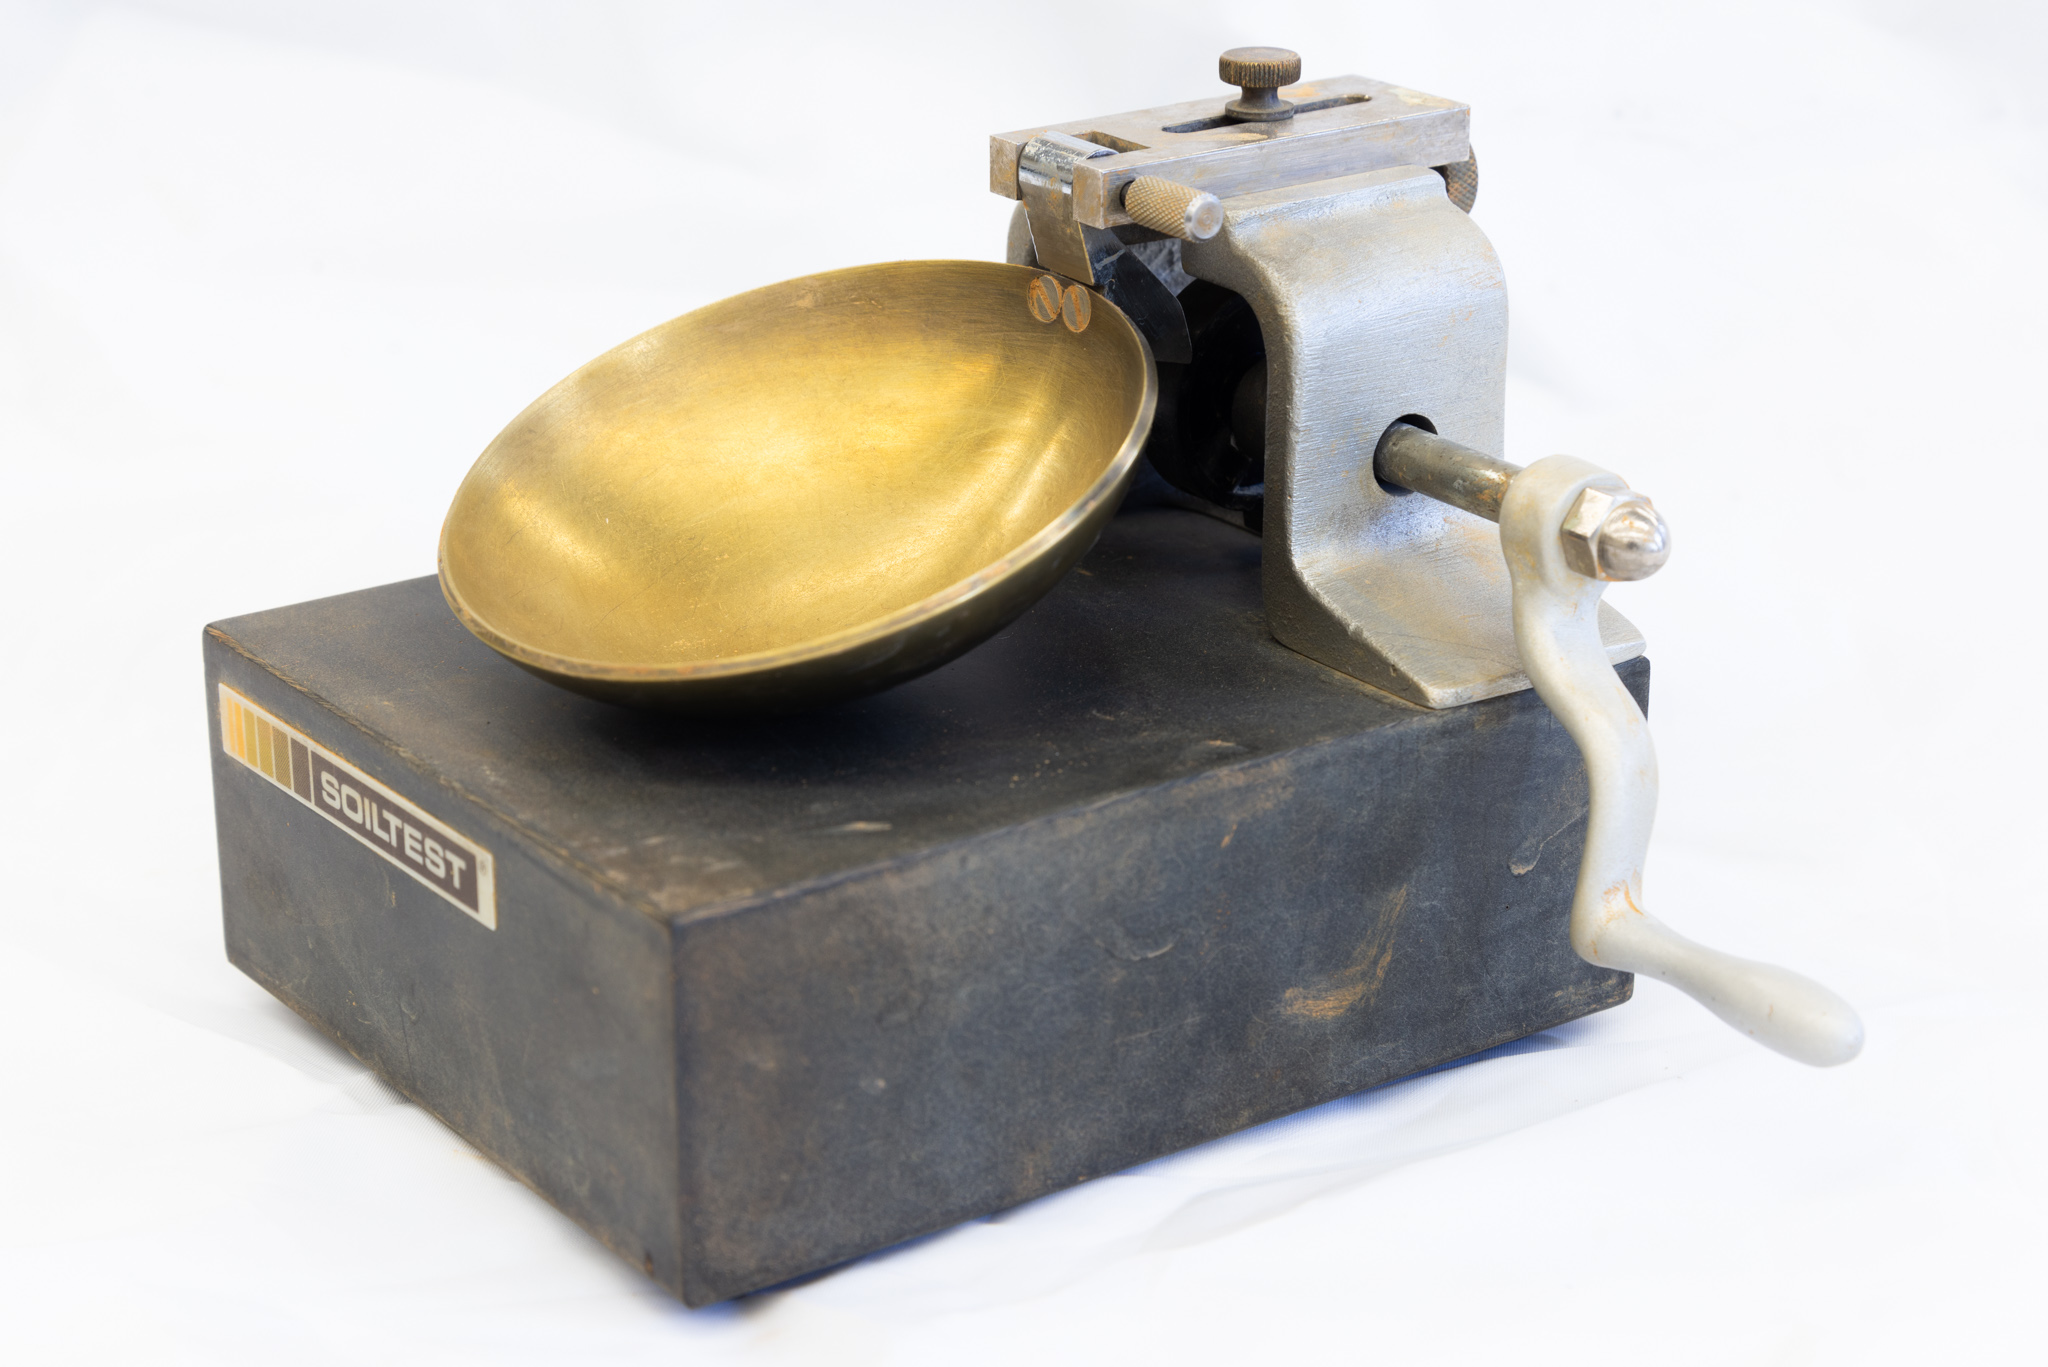
\includegraphics[width=0.8\textwidth]{GEO_5747.jpg}
    \caption{Example of a manually operated Casagrande cup. The crank is rotated counter-clockwise to lift and drop the brass bowl to impart a small but repeatable impact force into the specimen.}
    \label{fig:casagrandecup}
\end{figure}

\subsubsection{Preparation}
There are two critical pieces of equipment necessary to complete the liquid limit test: a grooving tool (Fig. \ref{fig:groovingtool}) and a hand-operated Casagrande cup setup. There are mechanical Casagrande cup setups that perform the test automatically, however for this exercise you will use the hand-operated version. While ASTM D4318 \S10 requires the verification of the Casagrande cup assembly, you may assume the assembly provided to you has been verified. Additionally, you will need three sample containers so that the moisture content can be determined. 

\begin{figure}[H]
    \centering
    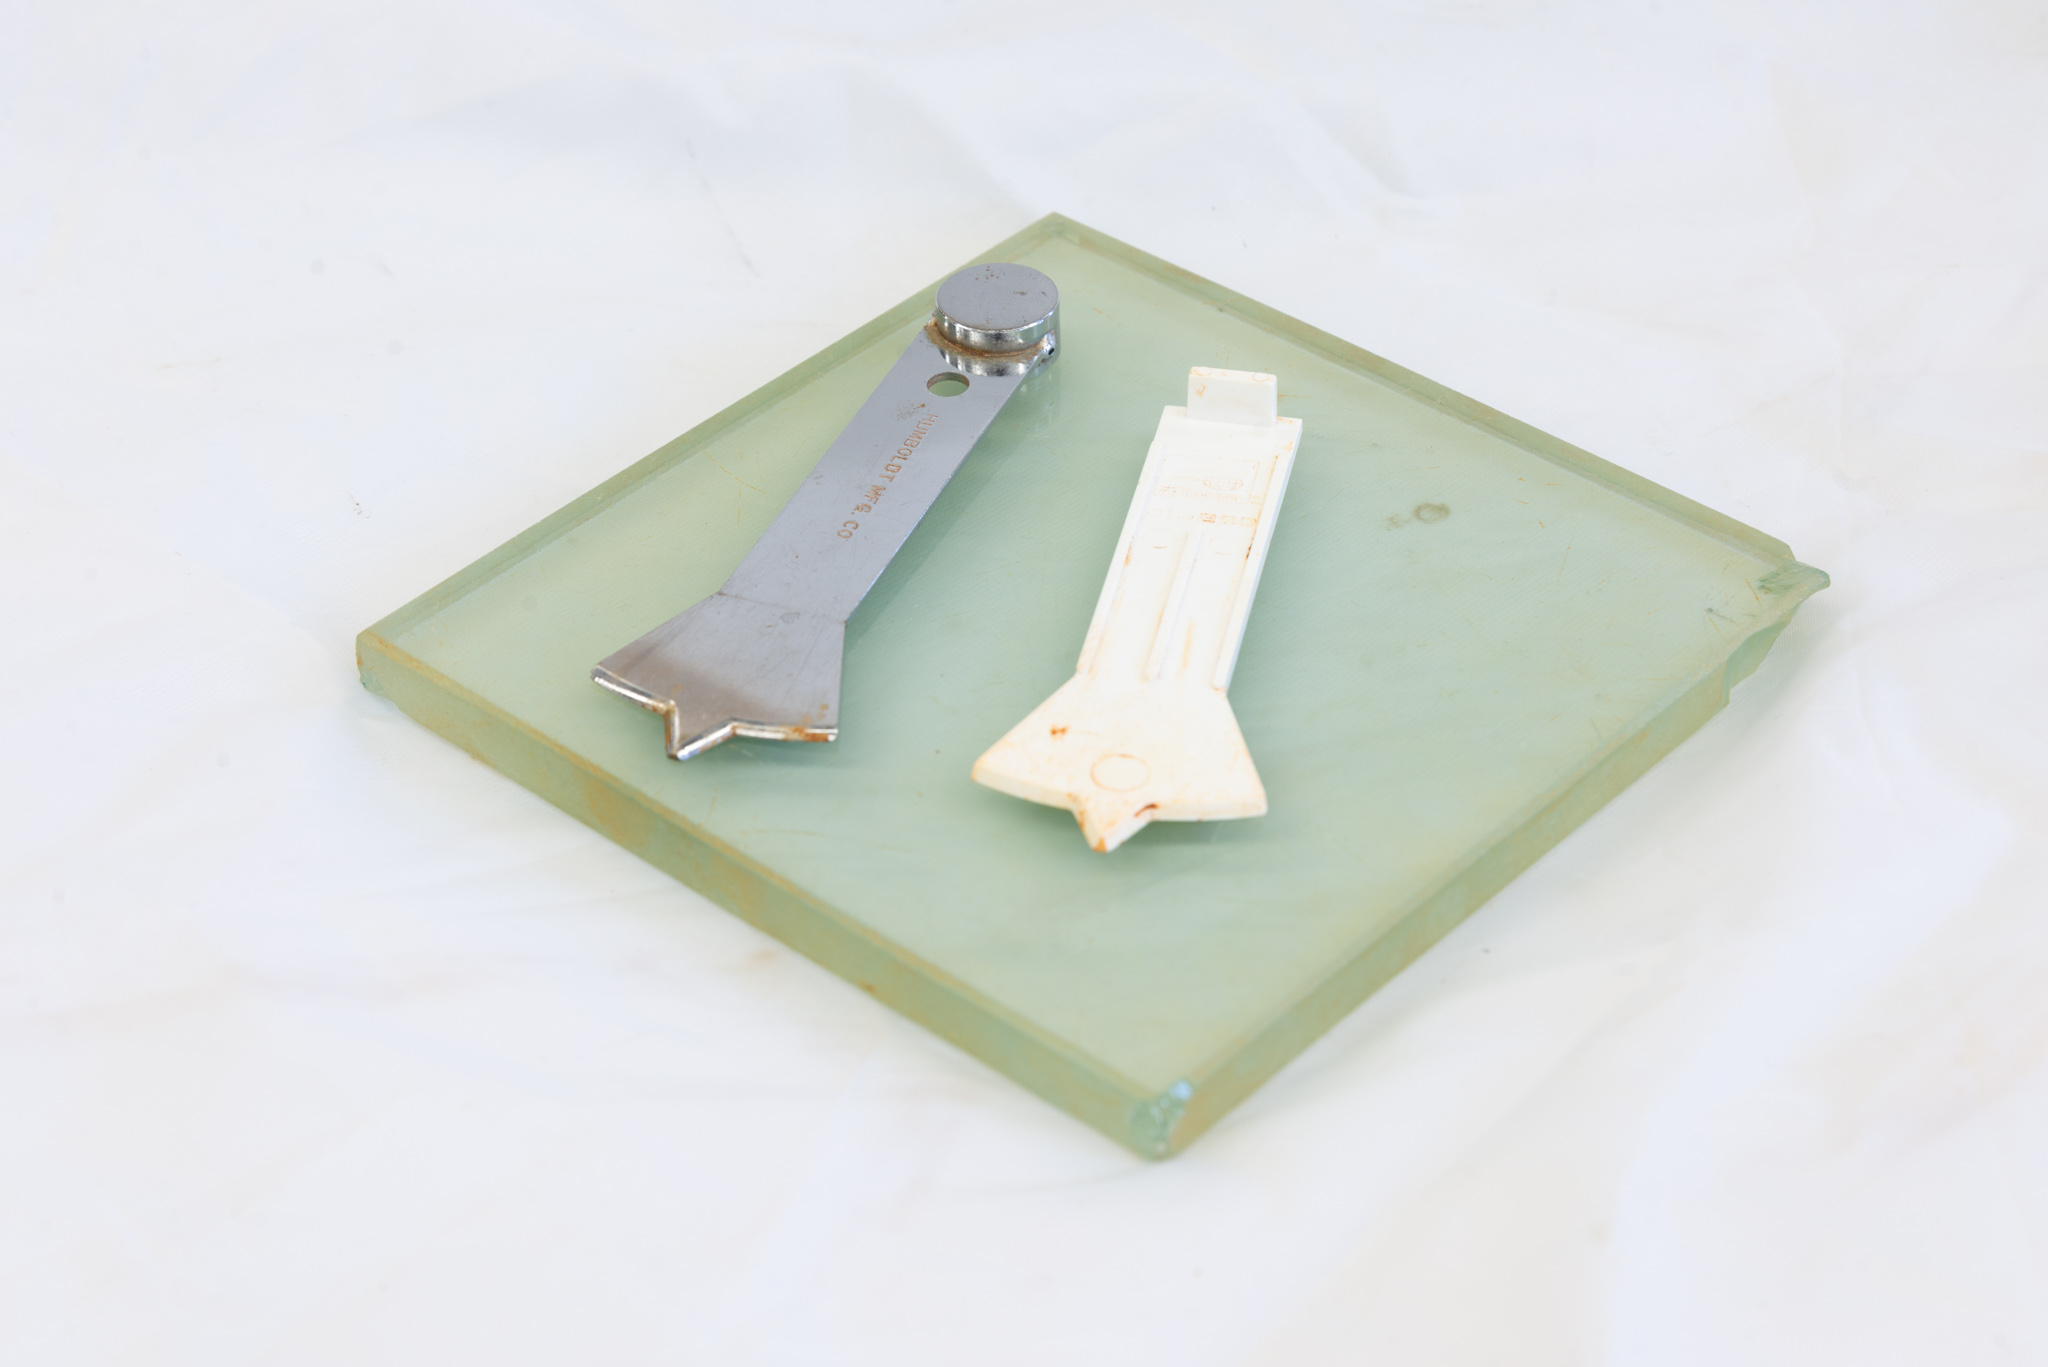
\includegraphics[width=0.8\textwidth]{GEO_5748.jpg}
    \caption{Example of plastic and metal grooving tools for use in the Casagrande cup. There is a different type of grooving tool that can also be used but will not be utilized for this laboratory exercise.}
    \label{fig:groovingtool}
\end{figure}

The most difficult part of the preparation is the soil sampling process. You want to start with the soil sample at a moisture state that will close the gap with 25 to 35 blows. For someone with no experience with this test, it can be nearly impossible to estimate this and a significant amount of time will be wasted attempting to achieve the correct starting moisture state. A previously prepared sample will be provided for you to start with.

You will be performing three tests at different moisture contents. To determine the precise moisture content for each test, the sample will be oven dried in a container. Measure the empty weights of the three sample containers and label them with sufficient detail that you can identify them at a later time.

\subsubsection*{Preparation Checklist}
\begin{itemize}
    \item Obtain liquid limit bowl apparatus and grooving tool
    \item Obtain previously prepared soil
    \item Obtain the empty weight of the three sample containers and label them
\end{itemize}

\subsubsection{Execution}
We will be performing the multi-point method as outlined in ASTM D4318 \S12. You will take a sample of the previously prepared soil and place it into the Casagrande cup. We are looking to achieve a horizontal surface, with respect to the ground, noting that the bowl sits at an angle. The depth at the deepest point in the bowl should be approximately 10 mm. Observe the surface for any air bubbles and attempt to eliminate them with as few pats as possible. If the sample is patted excessively, it will start to bleed water and will significantly affect the test result.

Once the soil pat is ready, groove it down the center with the grooving tool. The beveled edge of the tool should face you as you start at the back of the sample and pull towards you. The tool should be held perpendicular the entire time noting that the bowl is at an angle different than the table. It should take only one attempt to groove the soil pat. Do not groove the same sample multiple times as this may cause bleed water to form.

After the groove is formed, rotate the crank on the bowl at a rate of approximately 2 revolutions per second. Be sure to count the number of rotations, or drops, applied. Once the groove has closed to a length of approximately 13 mm, stop the test and record the number of drops.

Obtain a strip of the sample that includes a portion of the grooved section. Place in the sample container and record the weight. This sample will be oven dried overnight and you will be provided with the data at a later time.

Depending on the number of drops it took the first specimen to close, the remaining two samples may need additional water or to be dried. Ideally, the three tests would have a sample from each of the following ranges: 25--35, 20--30, and 15--25. As the water content increases, the number of drops required to close the groove decreases. So, if your first sample took 27 drops to close the groove, your next two tests should have increasing water contents. You typically would vary the water content by a single percent. So, if your first sample had a starting water content of 62\%, your next two samples should probably have water contents of 63\% and 64\%.

You will repeat the bowl drop procedure for the remaining two moisture contents. Remember to obtain a sample of each specimen in order to determine the exact moisture content.

\subsubsection*{Execution Checklist}
\begin{itemize}
    \item Record the number of drops required to close the gap of the three samples
    \item Record the estimated moisture contents for all three samples
    \item Record the weight of the obtained sample from each test run prior to oven drying
\end{itemize}

\subsubsection{Analysis}
The analysis phase is similar to the plastic limit test in that it is straightforward. However, a chart is involved in the analysis of liquid limit data. Once you have obtained your oven dry weight for the three samples, calculate the actual moisture content for each sample.

You will then plot your calculated moisture content versus number of drops required to close the groove. However, the x-axis (i.e. number of drops) should be plotted on a log scale, but the moisture content plotted on a arithmetical (i.e. linear) scale. Once plotted, apply a linear fit. The liquid limit is taken as the moisture content necessary to close the groove with exactly 25 drops. We round the moisture content to the nearest whole percent. For the example below (Fig. \ref{fig:exampleLL}), the liquid limit would be 44.

\begin{figure}[H]
    \centering
    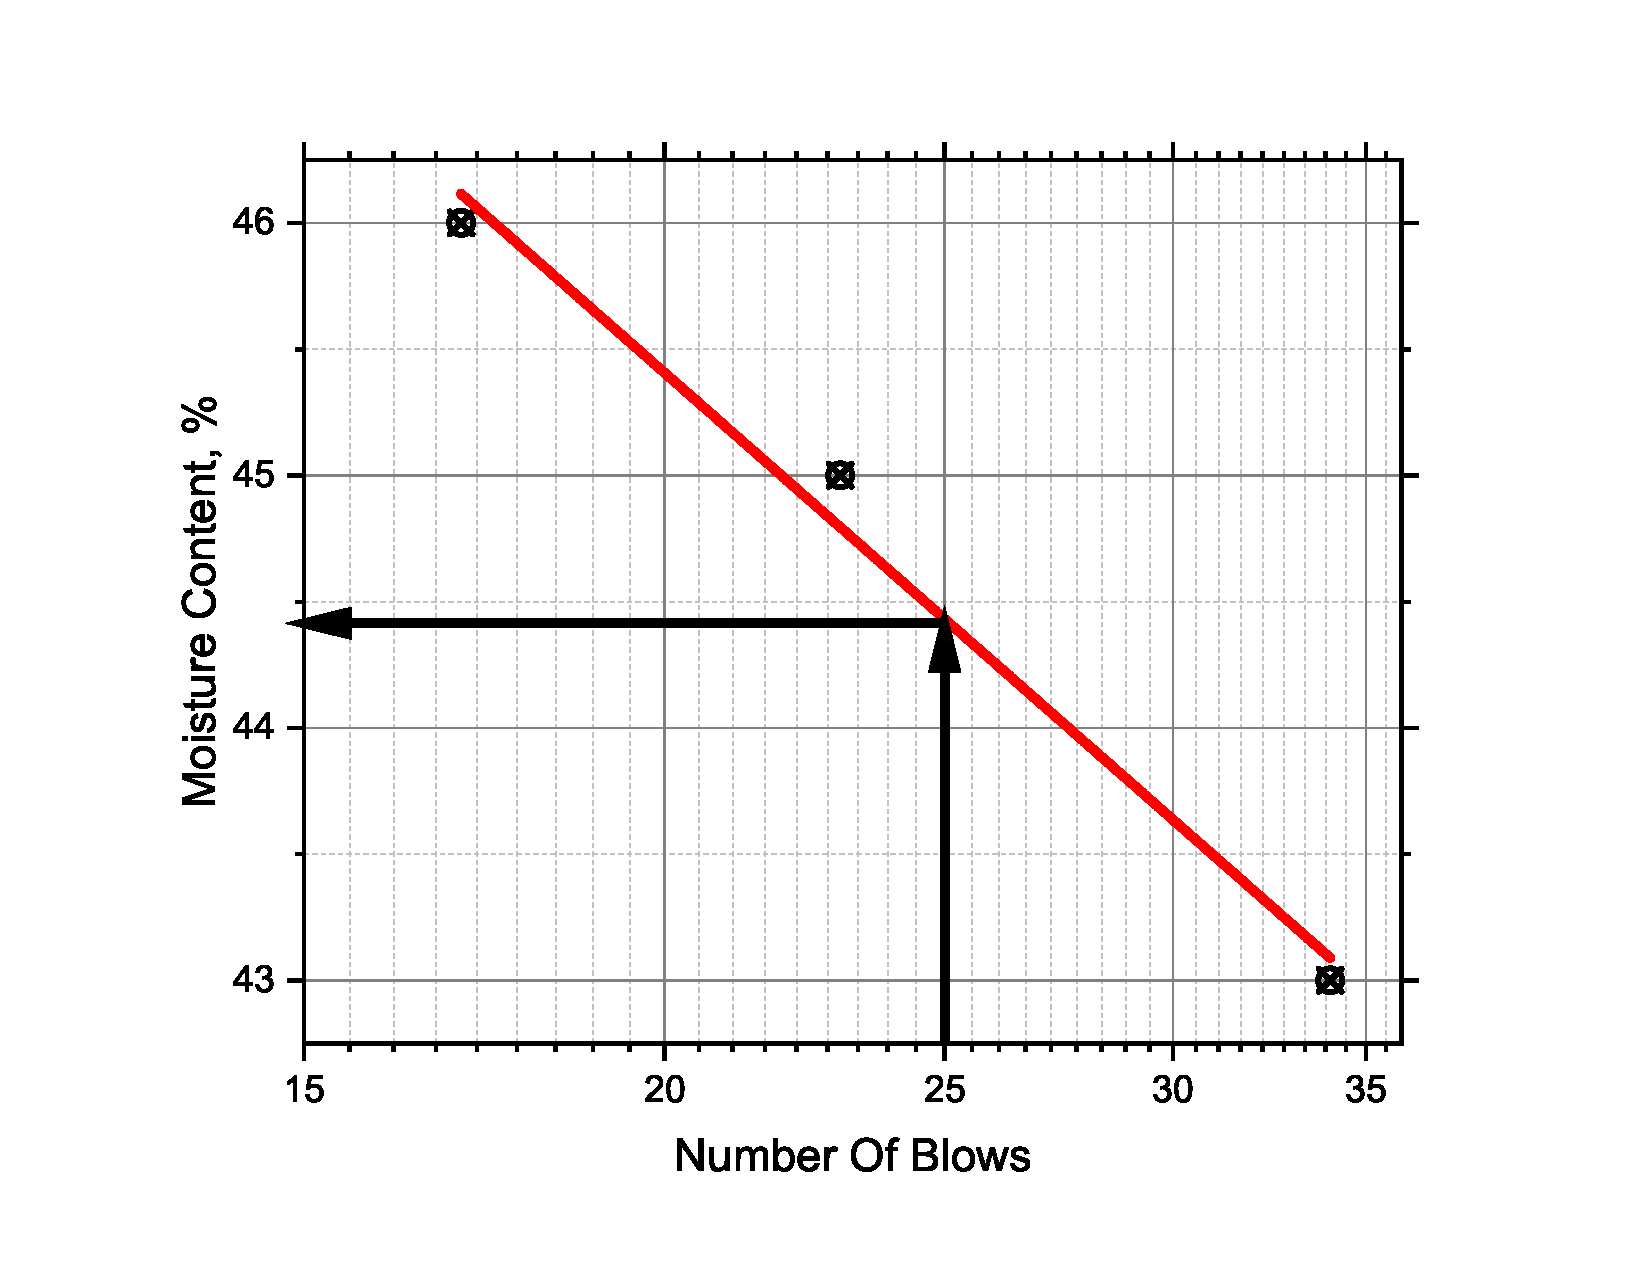
\includegraphics[width=0.8\textwidth]{Graph1.eps}
    \caption{Example of liquid limit plot. The x-axis is plotted on a log scale while the y-axis is plotted on a arithmetical (i.e. linear) scale. The liquid limit is taken as the moisture content necessary to close the groove with exactly 25 drops.}
    \label{fig:exampleLL}
\end{figure}

\subsubsection*{Analysis Checklist}
\begin{itemize}
    \item Calculate the true moisture contents for the three samples
    \item Plot the corresponding data
    \item Determine the liquid limit to the nearest whole percent
\end{itemize}

\subsection{Summary}
You have successfully run a liquid limit test. The liquid limit, combined with the plastic limit previously described, provides geotechnical engineers with critical information about the behavior of a soil and aids in the classification process. While the test procedure may seem ``weird'' or unusual, it is surprisingly repeatable for most soil types.

\pagebreak
\section{Deliverables}
For this laboratory exercise, the deliverables are quite simple. We just need the plastic limit, liquid limit, and plasticity index\footnote{This calculation was covered in lecture and is simply the liquid limit minus the plastic limit}. However, in certain geotechnical reports, you would be required to ``show your work''. An example of the required ``work'' to be shown is provided in Appendix A. At a minimum, your deliverable should contain:
\begin{itemize}
    \item Empty (i.e. tare) weight of the sample cans
    \item Weight of moist soil
    \item Weight of dry soil
    \item Moisture content of soil
    \item For LL, number of blows associated with the moisture content
    \item Chart showing calculation of LL value, as described in Fig. \ref{fig:exampleLL}
\end{itemize}

You should easily be able to fit all the required information on a single page. A large part of this exercise is professional formatting. You will likely spend more time making the page(s) look good than performing the actual calculations and this is okay! Professional engineers will typically use software specifically designed to make nice sheets. However, there are still some firms and engineers that do it manually. Most of the time the entire page is created in MS Excel due to the insane number of rows and columns needed. Here are some DOs and DON'Ts to help guide you in making a professional submission:

\begin{itemize}
    \item DO be consistent with decimal places and where applicable, follow the ASTM rules for number of decimal places
    \item DO indicate units properly
    \item DON'T use a font size smaller than 10pt
    \item DON'T use shading (i.e. shading alternating rows)
\end{itemize}

%\section*{References}
%\addcontentsline{toc}{section}{References}
%\bibliographystyle{techpubs}
%\bibliography{References}

%%%%%%%%%%%%%%%%%%%%%%%%%%%%%%%%%%%%%%%%%%%%%%%%%%%%%%%%%%%%%%%%%%%%
%   Please use the techpubs BibTeX style when compiling bibliography, or follow the instructions on tinyurl.com/techpubsnist to format your .bib / .bbl file appropriately.
%%%%%%%%%%%%%%%%%%%%%%%%%%%%%%%%%%%%%%%%%%%%%%%%%%%%%%%%%%%%%%%%%%%%
\pagebreak

\section*{Appendix A: Example Atterberg Limits Worksheet}
\label{AppendixA}
\addcontentsline{toc}{section}{Appendix A: Example Atterberg Limits Worksheet}
\begin{center}
    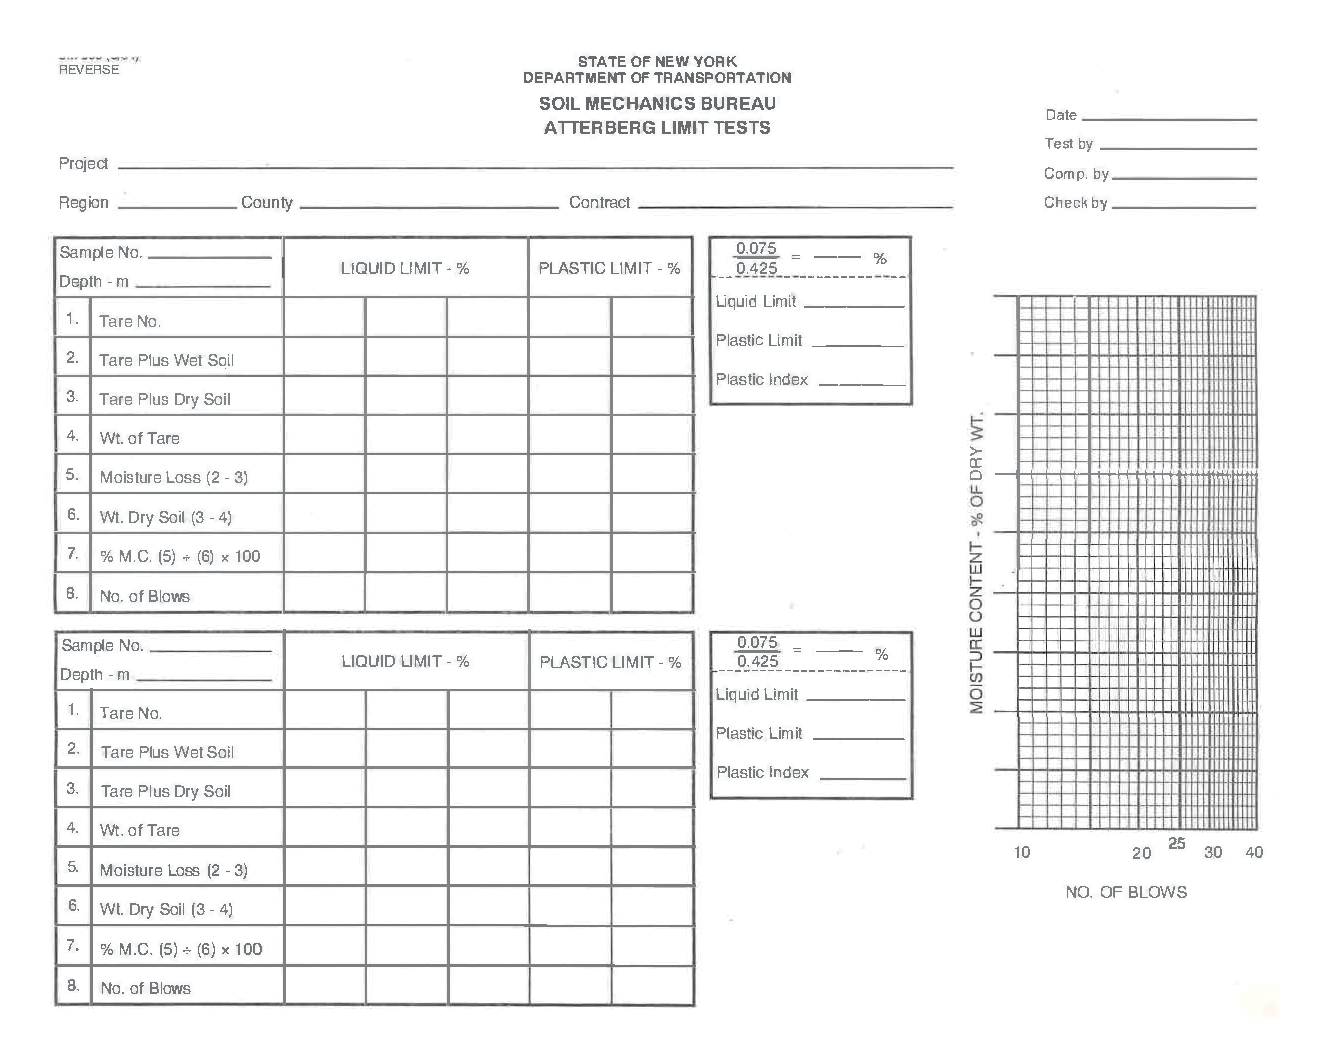
\includegraphics[width=1\linewidth]{GTM-7b24.eps}
\end{center}

%\pagebreak
%\section*{Appendix B: Change Log}
%\addcontentsline{toc}{section}{Appendix B: Change Log}
%This document was originally created on April 16, 2020. Any changes will be documented in this appendix.

\end{document}
%%%%%%%%%%%%%%%%%%%%%%%%%%%%%%%%%%%%%%%%%%%%%%%%%%%%%%%%%%%%%%%%%%%%
%   When referring to references in the text parenthetically, 
%	use the form “[1].” For example, “As Jones and Smith have shown [1];”
%	 however, when a reference is referred to non-parenthetically, use the form 
%	“. . . Ref. [1] . . .” (except at the beginning of a sentence where
%	“Reference [1] . . .” is the correct form).
%%%%%%%%%%%%%%%%%%%%%%%%%%%%%%%%%%%%%%%%%%%%%%%%%%%%%%%%%%%%%%%%%%%%

%%%%%%%%%%%%%%%%%%%%%%%%%%%%%%%%%%%%%%%%%%%%%%%%%%%%%%%%%%%%%%%%%%%%
%   Section references are “Sec. X”.
% 	“Section X” is used at beginning of sentence. 
%%%%%%%%%%%%%%%%%%%%%%%%%%%%%%%%%%%%%%%%%%%%%%%%%%%%%%%%%%%%%%%%%%%%

%%%%%%%%%%%%%%%%%%%%%%%%%%%%%%%%%%%%%%%%%%%%%%%%%%%%%%%%%%%%%%%%%%%%
%   Equation references are “Eq. (X)”.
% 	“Equation (1) is used at beginning of sentence.
%	Equations are numbered (#) on the right, per the standard LaTeX format
%%%%%%%%%%%%%%%%%%%%%%%%%%%%%%%%%%%%%%%%%%%%%%%%%%%%%%%%%%%%%%%%%%%%

%%%%%%%%%%%%%%%%%%%%%%%%%%%%%%%%%%%%%%%%%%%%%%%%%%%%%%%%%%%%%%%%%%%%
%   Tables should appear after they are mentioned in the text. 
%	Superscripted letters (a, b, c, etc.) should be used for table footnotes.
%%%%%%%%%%%%%%%%%%%%%%%%%%%%%%%%%%%%%%%%%%%%%%%%%%%%%%%%%%%%%%%%%%%%

%%%%%%%%%%%%%%%%%%%%%%%%%%%%%%%%%%%%%%%%%%%%%%%%%%%%%%%%%%%%%%%%%%%%
%   Figure references are “Fig. X”.
% 	“Figure X” is used at beginning of sentence. 
% 	Figures should appear after they are mentioned in the text.
%	Figures must have embedded alternate text or “alt text” in order 
%	to comply with Section 508 accessibility standards. 
%%%%%%%%%%%%%%%%%%%%%%%%%%%%%%%%%%%%%%%%%%%%%%%%%%%%%%%%%%%%%%%%%%%%